\documentclass[rmp,aps,twocolumn]{revtex4-1}

\usepackage[backref,breaklinks,colorlinks,citecolor=blue]{hyperref}  
\usepackage[all]{hypcap}
\usepackage{amsmath}
\usepackage{amssymb}
\usepackage{graphicx}
\usepackage{color}
\usepackage{natbib}
\usepackage{xspace}
\usepackage{nicefrac}
\usepackage[dvipsnames]{xcolor}
\usepackage[T1]{fontenc}
\usepackage{lmodern}
\usepackage{tablefootnote}
\usepackage{ulem}
\newcommand\myshade{85}
\colorlet{mycitecolor}{Turquoise}
\colorlet{mylinkcolor}{Turquoise}
\hypersetup{
 citecolor = mycitecolor!\myshade!black,
 linkcolor = mylinkcolor!\myshade!black,
 colorlinks = true,
}


\newcommand{\todo}[1]{\textcolor{red}{#1}}
\newcommand{\tocheck}[1]{\textcolor{green}{[Check:] #1}}
\newcommand{\citeme}{{\color{blue} CITE ME!}}
\newcommand{\ilya}[1]{\textcolor{magenta}{#1}}


\def\be{\begin{equation}}
\def\ee{\end{equation}}
\def\ba{\begin{eqnarray}}
\def\ea{\end{eqnarray}}

\begin{document}

\title{A 100 million year old thermometer}

\author{All author names to be added like this:\\}

\author{Ilya Mandel}
\email{imandel@star.sr.bham.ac.uk}
\affiliation{Institute of Gravitational Wave Astronomy and School of Physics and Astronomy, University of Birmingham, Edgbaston, Birmingham B15 2TT, United Kingdom}
%\\ and\\ Monash Centre for Astrophysics, School of Physics and Astronomy, Monash University, Clayton, Victoria 3800, Australia}

\begin{abstract}

GDGTs in ocean-floor sediments provide a fossil record of ocean temperatures in the distant past.  Previous efforts to calibrate temperature prediction based on modern GDGT data have been suboptimal.  We apply modern machine-learning tools to the problem of calibrating a temperature predictor based on GDGT data.

\end{abstract}

\maketitle

\section{Introduction}


We wish to make the following three key points:

\begin{itemize}

\item Even the modern GDGT data set is fundamentally imperfect at being a predictor for temperature;

\item We discuss how best to predict temperature from GDGT observations using the modern data set for calibration, using all available data without pre-judgement;

\item We analyse the prospects for applingy tools calibrated on the modern data set to cretaceous and eocene data.

\end{itemize}


\section{Data}

Others should describe the data set.

\section{Temperature prediction: calibration and validation}

\subsection{Nearest neighbours}

We begin by considering an agnostic approach to using some combination of the six observables (GDGT-0, GDGT-1, GDGT-2, GDGT-3, Cren and Cren-isomer, all of which we will jointly refer to as GDGTs) to predict temperature.  Whatever functional form the predictor might take, it can only provide accurate temperature predictions if nearby points in the six-dimensional observable space can be translated to nearby points in temperature space.  Conversely, if nearby points in the observable space correspond to vastly different temperatures, then no predictor will be able to provide a useful temperature estimate.

We therefore consider the prediction that would be offered by the the temperature at the nearest point in the parameter space.  Of course, nearness is a function of some distance metric on the space: e.g., it may be that the temperature is very sensitive to one observable, so even a small change in that observable corresponds to a significant distance, and rather insensitive to another, meaning that even with a large difference in the nominal value of that observable the distance is insignificant.  We will return to this later.  For now, we consider a very simple Euclidian distance estimate $D$ where the distance along each observable is normalised by the total spread in that observable across the entire data set.  This normalisation ensures that a dimensionless distance estimate can be produced even when observables have very different dynamical ranges, or even different units.  Thus, the normalised distance $D$ between parameter data points $x$ and $y$ is
\be\label{eq:dist}
D_{x,y}^2 \equiv \sum_{i=0}^{6} \frac{(GDGT_{i} (x) - GDGT_{i} (y) )^2}{var(GDGT_{i}} \, .
\ee
We show the distribution of nearest distances of points in the modern data set (excluding the sample itself) in \autoref{fig:nearest}.  

\begin{figure}
	\centering
	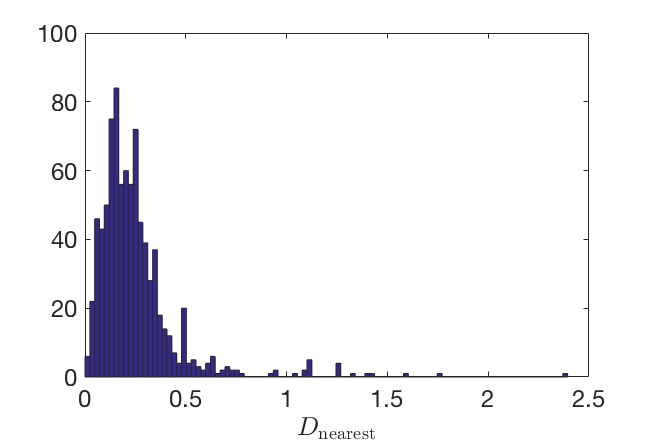
\includegraphics[width=0.5\textwidth]{nearest.png}
	\caption{\label{fig:nearest}  A histogram of the normalised distance to the nearest neighbour in GDGT space.}
\end{figure}

In order to enable meaningful comparison between temperature predictors, we will use the following consistent procedure for evaluating all predictors throughout this paper.  We divide the data set of 854 data points into 85 validation data points (chosen randomly) and 769 calibration points.  We calibrate the predictor on the calibration points, and then judge its performance on the calibration points using the square root of the average of the square of the difference between the prediction at each validation point and the true temperature value there:
\be\label{eq:pred}
\delta T = \sqrt{\frac{1}{N_v-1}\sum_{k=1}^{N_v} (\hat{T} (x_k) - T(x_k))^2},
\ee
where the sum is taken over each of $N_v=85$ validation points, $T$ is the known measured temperature (which we refer to as the true temperature) and $\hat{T}$ is the predicted temperature.  For conciseness, we will refer to $\delta T$ as the predictor standard error.  It is useful to compare the accuracy of the predictor to the standard deviation of all temperatures in the data set $\sigma T$, which corresponds to using the mean temperature as the predictor in \autoref{eq:pred}; for the modern data set, $\sigma T = 10.0$ degrees.  The so-called coefficient of determination $R^2$, given by 
\be
R^2 \equiv 1 - \left(\frac{\delta T}{\sigma T}\right)^2,
\ee
provides a measure of the fraction of the fluctuation in the temperature explained by the predictor.  We repeat the calibration--validation procedure for 10 randomly choices of the validation point subset, while using the same validation subsets for all predictor performance analyses.

The nearest-sample temperature predictor is $\hat{T}_\textrm{nearest} (x) = T(y)$ where $y$ is the nearest point to $x$ over the calibration data set, i.e., one that minimises $D_{x,y}$.  Figure \ref{fig:Tnearest} shows the scatter in the predicted temperature when using the temperature of the nearest data point to make the prediction.  Some of the extreme scatter indicates outliers in the data; we discusses these in \autoref{sec:discussion}.  Overall, the failure of the nearest-neighbour predictor to provide accurate temperature estimates even when the normalised distance to the nearest point is small, $D_\mathrm{nearest} \lesssim 0.5$, casts doubt on the possibility of designing an accurate predictor for temperature based on GDGT observations.  This could be due to significant measurement uncertainties, such as \tocheck{ad-hoc choices in measuring GDGTs associated with arbitrary placements of boundaries on spectrum readouts}.  Alternatively, it could be that GDGTs just are not able to explain temperature very well on their own: there might be contamination from other GDGT sources, or there could be other important bits of information we are not including in the analysis (even with very accurate data and the best statistical tools, the citation counts on papers published in this journal are unlikely to be accurately predicted by the weather patterns in Birmingham on the date of publication).   

\begin{figure}
	\centering
	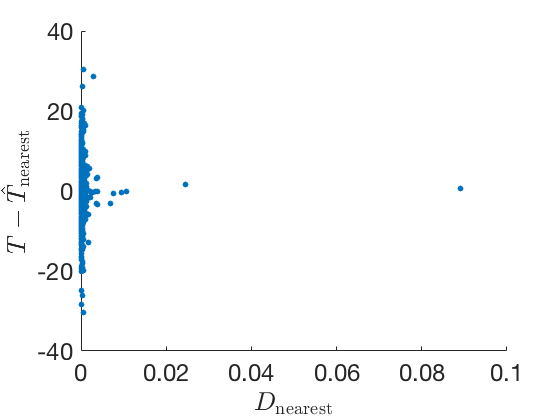
\includegraphics[width=0.5\textwidth]{Tnearest.png}
	\caption{\label{fig:Tnearest}  The standard error of the nearest-neighbour temperature predictor as a function of the distance to the nearest calibration sample.}
\end{figure}

On the other hand, the standard error for the nearest-neighbour temperature predictor is $\delta T_\mathrm{nearest} = 4.5$ degrees.  This is less than half of the standard deviation $\sigma T$ in the temperature values across the modern data set. Thus, the temperatures corresponding to nearby points in GDGT observable space also cluster in temperature space.  Consequently, there is hope that we can make some useful if imperfect temperature predictions.  The value of $\delta T_\mathrm{nearest}$ will also serve as a useful benchmark in this design: while we may hope to do better by, say, suitably averaging over multiple nearby calibration points rather than adopting the temperature at one nearest point as a predictor, any method that performs worse than the nearest-neighbour predictor is clearly suboptimal. 

\subsection{TEX$_{86}$}

A particular combination of GDGTs known as TEX$_{86}$ has been regularly used as the basis for making temperature predictions \citeme.  This is defined as 
\be\label{eq:TEX86}
\mathrm{TEX}_{86} = \frac{\mathrm{GDGT}_2+\mathrm{GDGT}_3+\mathrm{Cren}'}{\mathrm{GDGT}_1+\mathrm{GDGT}_2+\mathrm{GDGT}_3+\mathrm{Cren}'}\, .
\ee
TEX$_{86}$ reduces the six-dimensional observable space to a single number.  While this has the advantage of convenience for manipulation and simple analytic formulae for predictors, as illustrated below, this approach has one critical disadvantage: it wastes the information embedded in hard-earned data.  Figure \ref{fig:TEX86} illustrates both the advantage and disadvantage of TEX$_{86}$.  On the one hand, there is a clear correlation between TEX$_{86}$ and the temperature (left panel of \autoref{fig:TEX86}), with a correlation coefficient of $0.81$ corresponding to an overwhelming statistical significance of $10^{-198}$.  On the other hand, very similar TEX$_{86}$ values can correspond to very different temperatures.  We can apply the nearest-neighbour temperature prediction approach to the TEX$_{86}$ value alone rather than the full GDGT parameter space; this predictor yields a large standard error of $\delta T_\mathrm{nearest TEX86} = 8.0$ degrees (right panel of \autoref{fig:TEX86}).  While smaller than $\sigma T$, this is significantly larger than $\delta T_\mathrm{nearest}$, consistent with the loss of information in TEX$_{86}$.  We therefore do not expect other predictors based on TEX$_{86}$ to perform as well as those based on the full available data set.

Indeed, this is what we find when we consider predictors of the form $\hat{T}_\mathrm{OneTEX}  = a + b / \mathrm{TEX}_{86}$ \citeme and $\hat{T}_\mathrm{TEXH}  = c + d \log \mathrm{TEX}_{86}$ \citeme.  We fit the free parameters $a, b, c, d$ by minimising the sum of squares of the residuals over the calibration data sets.  We find that \tocheck{$\delta T_\mathrm{OneTEX} = 6.1$ degrees} (note that this is slightly better than using the fixed values of $a$ and $b$ from \citeme, which would yield \tocheck{$\delta T_\mathrm{OneTEX} = 6.2$ degrees}.  Meanwhile \ilya{[Will, this is for you: ]} $\delta T_\mathrm{TEXH} = XXX$ degrees.  \ilya{[Should we also include TEXL?]}  

\ilya{[Will: this part about Bayespar is for you]} \citeme proposed a more sophisticated approach to obtaining the transfer function from TEX$_{86}$ to temperature ...  However, along with the simpler TEX$_{86}$--based models described above, this approach still suffers from the arbitrary reduction of a six-dimensional data set to a single number.  Therefore, it is not surprising that it performs more poorly than what could be achieved even with the simplest nearest-neighbour predictor using the full six-dimensional data set.

We now consider improvements on the nearest-neighbour predictor motivated by machine learning techniques.  






\subsection{Machine learning}

nearest temperature prediction.  


\section{Measuring temperature in the distant past}

\section{Discussion}\label{sec:discussion}

\begin{acknowledgements}
We thank the research councils for their munificence.

\end{acknowledgements}

\bibliographystyle{hapj}
\bibliography{paleo}

\end{document}


